\documentclass[a4paper, twoside]{report}

%%%%%%%%%%%%%%%%%%%%%%%%%%%%%%%%%%%%%%%
%%%%%%%%%%%%% IMPORT PACKAGES %%%%%%%%%
%%%%%%%%%%%%%%%%%%%%%%%%%%%%%%%%%%%%%%%
\usepackage[hidelinks]{hyperref}
\usepackage{subfigure}
\usepackage{fancyvrb}
\usepackage{amsmath, amsfonts, amsthm, amssymb}
\usepackage{stmaryrd}
\usepackage{verbatim}
\usepackage{graphicx}
\usepackage{setspace}
\usepackage[ruled, vlined]{algorithm2e}
\graphicspath{{Figures/}}

%%%%%%%%%%%%%%%%%%%%%%%%%%%%%%%%%%%%%%%5
\usepackage{listings}
\usepackage{xcolor}
\definecolor{codegreen}{rgb}{0,0.6,0}
\definecolor{codegray}{rgb}{0.5,0.5,0.5}
\definecolor{codepurple}{rgb}{0.58,0,0.82}
\definecolor{backcolour}{rgb}{0.95,0.95,0.92}

\lstdefinestyle{mystyle}{
    backgroundcolor=\color{backcolour},   
    commentstyle=\color{codegreen},
    keywordstyle=\color{magenta},
    numberstyle=\tiny\color{codegray},
    stringstyle=\color{codepurple},
    basicstyle=\ttfamily\footnotesize,
    breakatwhitespace=false,         
    breaklines=true,                 
    captionpos=b,                    
    keepspaces=true,                 
    numbers=left,                    
    numbersep=5pt,                  
    showspaces=false,                
    showstringspaces=false,
    showtabs=false,                  
    tabsize=2
}
\lstset{style=mystyle}
%%%%%%%%%%%%%%%%%%%%%%%%%%%%%%%%%%%%%%%%
%%%%%%%%%%%%%%%%%%%%%%%%%
\newtheorem{theorem}{Theorem}[section]
\newtheorem{exa}{Example}[section]
\newtheorem{corollary}[theorem]{Corollary}
\newtheorem{lemma}[theorem]{Lemma}
\newtheorem{proposition}[theorem]{Proposition}

\theoremstyle{definition}
\newtheorem{definition}[theorem]{Definition}
\newtheorem{remark}[theorem]{Remark}
\newtheorem{notation}[theorem]{Notation}
\newtheorem{assumption}[theorem]{Assumption}
\newtheorem{conjecture}[theorem]{Conjecture}

\newcommand{\ind}{1\hspace{-2.1mm}{1}} %Indicator Function
\newcommand{\I}{\mathtt{i}}
\newcommand{\D}{\mathrm{d}}
\newcommand{\E}{\mathrm{e}}
\newcommand{\RR}{\mathbb{R}}
\newcommand{\sgn}{\mathrm{sgn}}
\newcommand{\atanh}{\mathrm{arctanh}}
\def\equalDistrib{\,{\buildrel \Delta \over =}\,}
\numberwithin{equation}{section}


%%%%%%%%%%%%%%%%%%%%%%%%%%%%%%%%%%%%%%%%%%%%%%%
%%%%%%%%%%%%%%%%%%%%%%%%%%%%%%%%%%%%%%%%%%%%%%%
%% Sets page size and margins
\usepackage[a4paper,top=3cm,bottom=2cm,left=3cm,right=3cm,marginparwidth=1.75cm]{geometry}
\title{Solving the Collatz conjecture}
\author{Ilia Sobakinskikh  (CID: 00000000)}

% for the confusion matrix: https://tex.stackexchange.com/a/20284
\usepackage{tikz}
\usetikzlibrary{positioning}



\begin{document}
\begin{titlepage}

\newcommand{\HRule}{\rule{\linewidth}{0.5mm}} 

\includegraphics[width=8cm]{logo.png}\\[1cm]
\center

\quad\\[1.5cm]
\textsc{\Large Imperial College London}\\[0.5cm]
\textsc{\large Department of Mathematics}\\[0.5cm]

\makeatletter
\HRule \\[0.2cm]
\begin{spacing}{2.5}
{\huge \bfseries \@title}
\end{spacing}
\HRule \\[1.5cm]
 
\begin{minipage}{0.8\textwidth}
\begin{flushleft} \large
\emph{Author:}
\@author
\end{flushleft}
\end{minipage}
~\vspace{2cm}
\makeatother


{\large A thesis submitted for the degree of}\\[0.5cm]
{\large \emph{MSc in Mathematics and Finance, 2022-2023}}\\[0.5cm]

\vfill

\end{titlepage}

\mbox{}\newline\vspace{10mm} \mbox{}\LARGE
%
{\bf Declaration} \normalsize \vspace{5mm}

The work contained in this thesis is my own work unless otherwise stated.

\newpage

\renewcommand{\abstractname}{Acknowledgements}
\begin{abstract}
    This is where you usually thank people who have provided useful assistance, feedback,...., during your project.
\end{abstract}

\newpage

\renewcommand{\abstractname}{Abstract}
\begin{abstract}
    The abstract is a short summary of the thesis' contents.
    It should be about half a page long and be accessible by someone not familiar with the project.
    The goal of the abstract is also to tease the reader and make him want to read the whole thesis.
\end{abstract}

\tableofcontents
\listoffigures
\listoftables






% %%%%%%%%%%%%%%%%%%%%%%%%%%%%%%%%%%%%%%%%%%%%%%%
% \begin{remark}
% Please bear in mind the following when writing your thesis (or anything for that matter):
% you are not writing for you. You are writing for an audience, who will (have to) read your work.
% Please be considerate, and explain everything clearly. 
% In this case, the audience could be your fellow MSc students, 
% with some general knowledge of the area, but maybe not specialised to your particular topic.
% \end{remark}


% \newpage
% %%%%%%%%%%%%%%%%%%%%%%%%%%%%%%%%%%%%%%%%%%%%%
% \chapter{How to write mathematics}\label{sec:HowTo}
% In this section, we show some examples of properly written mathematical expressions and sentences.
% In the header of your thesis, you can define \LaTeX \ shortcuts to write more quickly.


%%%%%%%%%%%%%%%%%%%%%%%%%%%%%%%%%%%%%%%%%%%%%%%
\chapter*{Introduction}

% The introduction is one of the most important components of the thesis.
% It should be readable by anyone, 
% including people without prior knowledge of the field.
% It should progressively introduce the main topic of the paper, and explain the structure of the thesis.
% In Section~\ref{sec:HowTo}, we shall provide several examples of clearly written examples,
% whereas Section~\ref{sec:WhatNotToDo} will gather a certain number of common mistakes and errors.

In this thesis, we explore how the inference time of a Transformer Neural Network can be efficiently optimized with applications to real-time anomaly detection in financial time series.
The financial time series are price series such as asset prices.
Unfortunately, the data is often with errors or outliers that make the downstream data processing tasks useless, unstable or even harmful \cite{Falkenberry_2008} \cite{Vallis_Hochenbaum_Twitter}. Moreover, the amount of financial time-series data has been significantly increasing \cite{AnomalyDataBig}.
Hence, there is a need for better data-cleaning methods in terms of accuracy and in terms of processing speed.

Transformers as a neural network architecture have achieved superior performances in many tasks such as Natural Language Processing and Computer Vision \cite{TransformersNLP}.
Time series modelling and especially anomaly detection tasks can benefit from the features of transformers architecture in multiple ways, including the capacity to capture long-range dependencies and interactions \cite{2202.07125}.

Increasingly powerful hardware, such as field-programmable gate arrays (FPGAs), have seen increasing usage in recent years due to their reconfigurability and high performance \cite{10.1007/978-3-319-56258-2_14}.

We explore different Transformer architectures for time series modelling and how they can be efficiently implemented on an FPGA board (PYNQ-Z2).
In particular, we examine the application of Transformers to detect anomalies in time series and we show how they can be efficiently implemented on an FPGA board to minimize latency or to maximize throughput.


%%%%%%%%%%%%%%%%%%%%%%%%%%%%%%%%%%%%%%%%%%%%%%%
\chapter{Methodology}

In this chapter, we will describe the main concepts and ideas used in this work.
The reader will be introduced to the main concepts of the Transformer architecture and how it can be used for anomaly detection in time series.
Finally, the main concepts of programming an FPGA will be introduced and the specific optimizations that can be applied to speed up the computations.

% TODO: use neurips paper as an example:
% https://proceedings.neurips.cc/paper_files/paper/2019/file/6775a0635c302542da2c32aa19d86be0-Paper.pdf

\section{Problem Formulation}


\begin{definition}
    We consider a \textbf{time-series} $\mathcal{T}$ which is simply a timestamped sequence of observations $x_i \in R^n$.
\end{definition}
\begin{remark}
    Most of the times we will consider univariate case, i.e. $n=1$.
    An example of this is a price time-series of a single stock.
    However, the multivariate case is also important and we will consider it in the experiments.
    For example, one can consider a time-series of prices of multiple stocks to get a multivariate time series.
\end{remark}


\begin{definition}
    The \textbf{Anomaly Detection} task:
    for any time-series $\hat{\mathcal{T}}$ of length $n$, we need to predict $\mathcal{Y} = \{y_1, . . . , y_n \}, y_i \in \{0, 1\}$,
    whether the datapoint at the $i$-th timestamp anomalous (where by convention we will use $1$ as anomaly and $0$ as not an anomaly).
\end{definition}
In this work, we will restrict ourselves to the \textbf{supervised case}
where the labels $y_i$ are known for the \emph{seen} (or training) part of the dataset.

\begin{remark}
    One can also consider an unsupervised task.
    However, one issue with the unsupervised task is that it is hard to evaluate
    the performance (i.e., accuracy) of the model's predictions \cite{1905.05667}.
\end{remark}


\section{Transformers}

In this section, we will describe the main concepts of the Transformer architecture.
We will describe the main building blocks of the Transformer architecture
and will give a special treatment to the attention mechanism firstly introduced in \cite{1409.0473}.

% TODO:
% https://ai.stackexchange.com/questions/23221/how-is-bert-different-from-the-original-transformer-architecture
% Both the encoder-decoder architecture and the attention mechanism are not novel proposals. In fact, previous neural network architectures to solve many NLP tasks, such as machine translation, had already used these mechanisms (for example, take a look at this paper). The novelty of the transformer and this cited paper is that it shows that we can simply use attention to solve tasks that involve sequences (such as machine translation) and we do not need recurrent connections, which is an advantage, given that recurrent connections can hinder the parallelization of the training process.

\subsubsection{General architecture}

In \cite{1706.03762}, authors introduced the Transformer architecture which a neural network architecture
which is the architecture that is dominantly used in Natural Language Processing tasks.
The architecture's main feature was reliance on the attention mechanism and the complete elimination
of recurrent and convolutional layers.

\begin{figure}[h!]
    \centering
    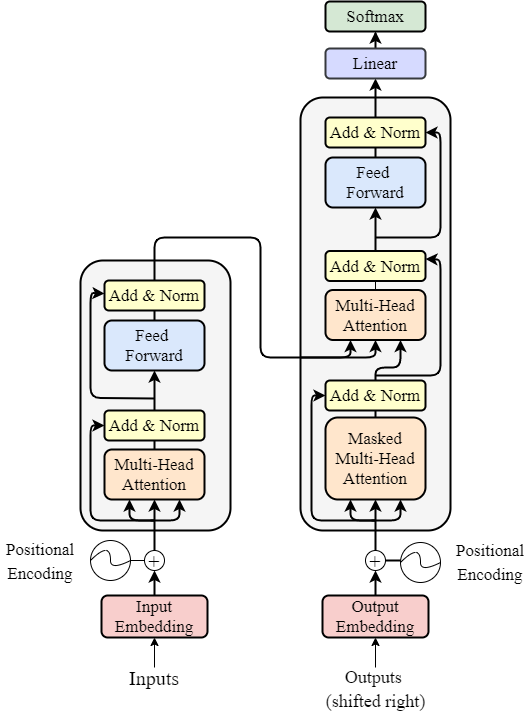
\includegraphics[scale=0.5]{attention_is_all_you_need.png}
    \caption{Model architecture of the Transformer \cite{1706.03762}}
    \label{fig:attention_is_all_you_need}
\end{figure}

Figure \ref{fig:attention_is_all_you_need} presents the main architecture of the transformer.
The architecture consists of an \textbf{encoder} and a \textbf{decoder}.
For the purpose of the thesis we will only consider the \textbf{encoder} part of the architecture.
% TODO: maybe describe the decoder also?
The \textbf{encoder} is preceded by a \textbf{positional encoding} layer which is used to \emph{inject} the positional information
to the input vectors $x_i$ because the attention mechanism is permutation invariant, this will be explained in Section \ref{sec:attention_mechanism}.

% TODO: explain positional encoding and why we need it
% https://uvadlc-notebooks.readthedocs.io/en/latest/tutorial_notebooks/tutorial6/Transformers_and_MHAttention.html

The \textbf{encoder} consists of $N$ identical layers. Each layer has two sub-layers which are a
\textbf{multi-head self-attention} layer and
a \textbf{feed-forward} layer.
The \textbf{feed-forward} layer $\text{FFN}(\cdot)$ is a simple fully-connected layer
with a non-linear activation function applied element-wise to the
result\footnote{
    In general, a \textbf{fully-connected} layer $\text{FC}(x)$ is simply a linear transformation inputs $X$ (i.e., a matrix multiplication) with the activation function applied element-wise to the result.
    That is, $\text{FC}(x)=f(W\cdot x + b)$ where $W$ is a weight matrix and $b$ is a bias vector and $f(\cdot)$ is the activation function.
    Authors of \cite{1706.03762} used the ReLU activation function
}.
Specifically, authors of \cite{1706.03762} used an $\text{FC}$ layer with
the ReLU activation function $$\text{ReLU}(x)=\max(0, x)$$
followed by another $\text{FC}$ layer without activation function, i.e.
$$\text{FFN}(x)=W_2 \cdot ReLU(W_1\cdot x+b_1)+b_2$$

The \textbf{Add \& Norm} layer is a residual connection \cite{1512.03385} followed by a layer normalization layers \cite{1607.06450}.
Those layers are not essential for this work and will not be described in detail.
% TODO: maybe describe them in appendix

This constitutes the main building block of the Transformer encoder architecture.
The next section will describe the attention mechanism in detail.


\subsection{Attention mechanism} \label{sec:attention_mechanism}

This section will describe the attention mechanism, its variations and the intuition behind it.
Moreover, we will compare different attention mechanism implementations in terms of
their computational complexity and their ability to capture long-range dependencies.
% basically, a survey...

\subsubsection{Dot-Product Attention and Multi-Head Attention}

% TODO: cite the common dot-product attention not as a scaled dot product attention
% https://lilianweng.github.io/posts/2018-06-24-attention/

The attention mechanism introduced in the Transformer architecture \cite{1706.03762} used a \textbf{scaled dot-product attention}.

% TODO: cite similarity to non-local filters
% Self-attention is a type of attention mechanism where the model
% makes prediction for one part of a data sample using other parts
% of the observation about the same sample. Conceptually, it feels quite similar
% to non-local means. Also note that self-attention is permutation-invariant;
% in other words, it is an operation on sets.

The main idea of the \textbf{dot-product attention} mechanism is to compute the mapping of a query $q_i$ for each input vector $x_i$ to a set of key-value pairs $(k_j, v_j)$.
The query $q_i$, key $k_i$ and value $v_i$ vectors are simply linear transformations of the input vectors $x_i$,
i.e., $q_i=W_Q\cdot x_i$, $k_i=W_K\cdot x_i$, $v_i=W_V\cdot x_i$ where $W_Q$, $W_K$ and $W_V$ are the weight matrices.
The attention mechanism is a weighted sum of the values $v_j$ where the weights are computed as a function of the query $q_i$ and the key $k_j$.
That is, $Attention(x_i)=\sum_j \alpha_{ij} v_j$ where $\alpha_{ij}=\text{softmax}(q_i \cdot v_i)$ is the weight of the $j$-th value $v_j$.
In practice, the attention mechanism is computed for all the queries $q_i$ at the same time by utilizing the following expression in matrix form:
\begin{equation}
    \begin{array}{rll}
        Q & = W_Q \cdot X, \\
        K & = W_K \cdot X, \\
        V & = W_V \cdot X
    \end{array}
\end{equation}
\begin{equation}\label{eq:dot_product_attention_matrix}
    \text{Attention}(Q, K, V)=\text{softmax}(Q K^T) V
\end{equation}

\begin{remark}
    In \cite{1706.03762}, authors additionally scaled the weights $\alpha_i$ by the square root of the dimension of the key vectors $d_k$.
    This is, however, not strictly necessary and is done for numerical stability reasons.
\end{remark}

The \textbf{multi-head attention} mechanism is simply a concatenation of multiple attention mechanisms.
That is, we can compute $h$ different attention mechanisms in parallel and then concatenate the results.
The main idea behind this is that different attention mechanisms can learn different features of the input vectors.

Figure \ref{fig:attention_is_all_you_need} visualizes the attention mechanism introduced in \cite{1706.03762}.

\begin{figure}[h!]
    \centering
    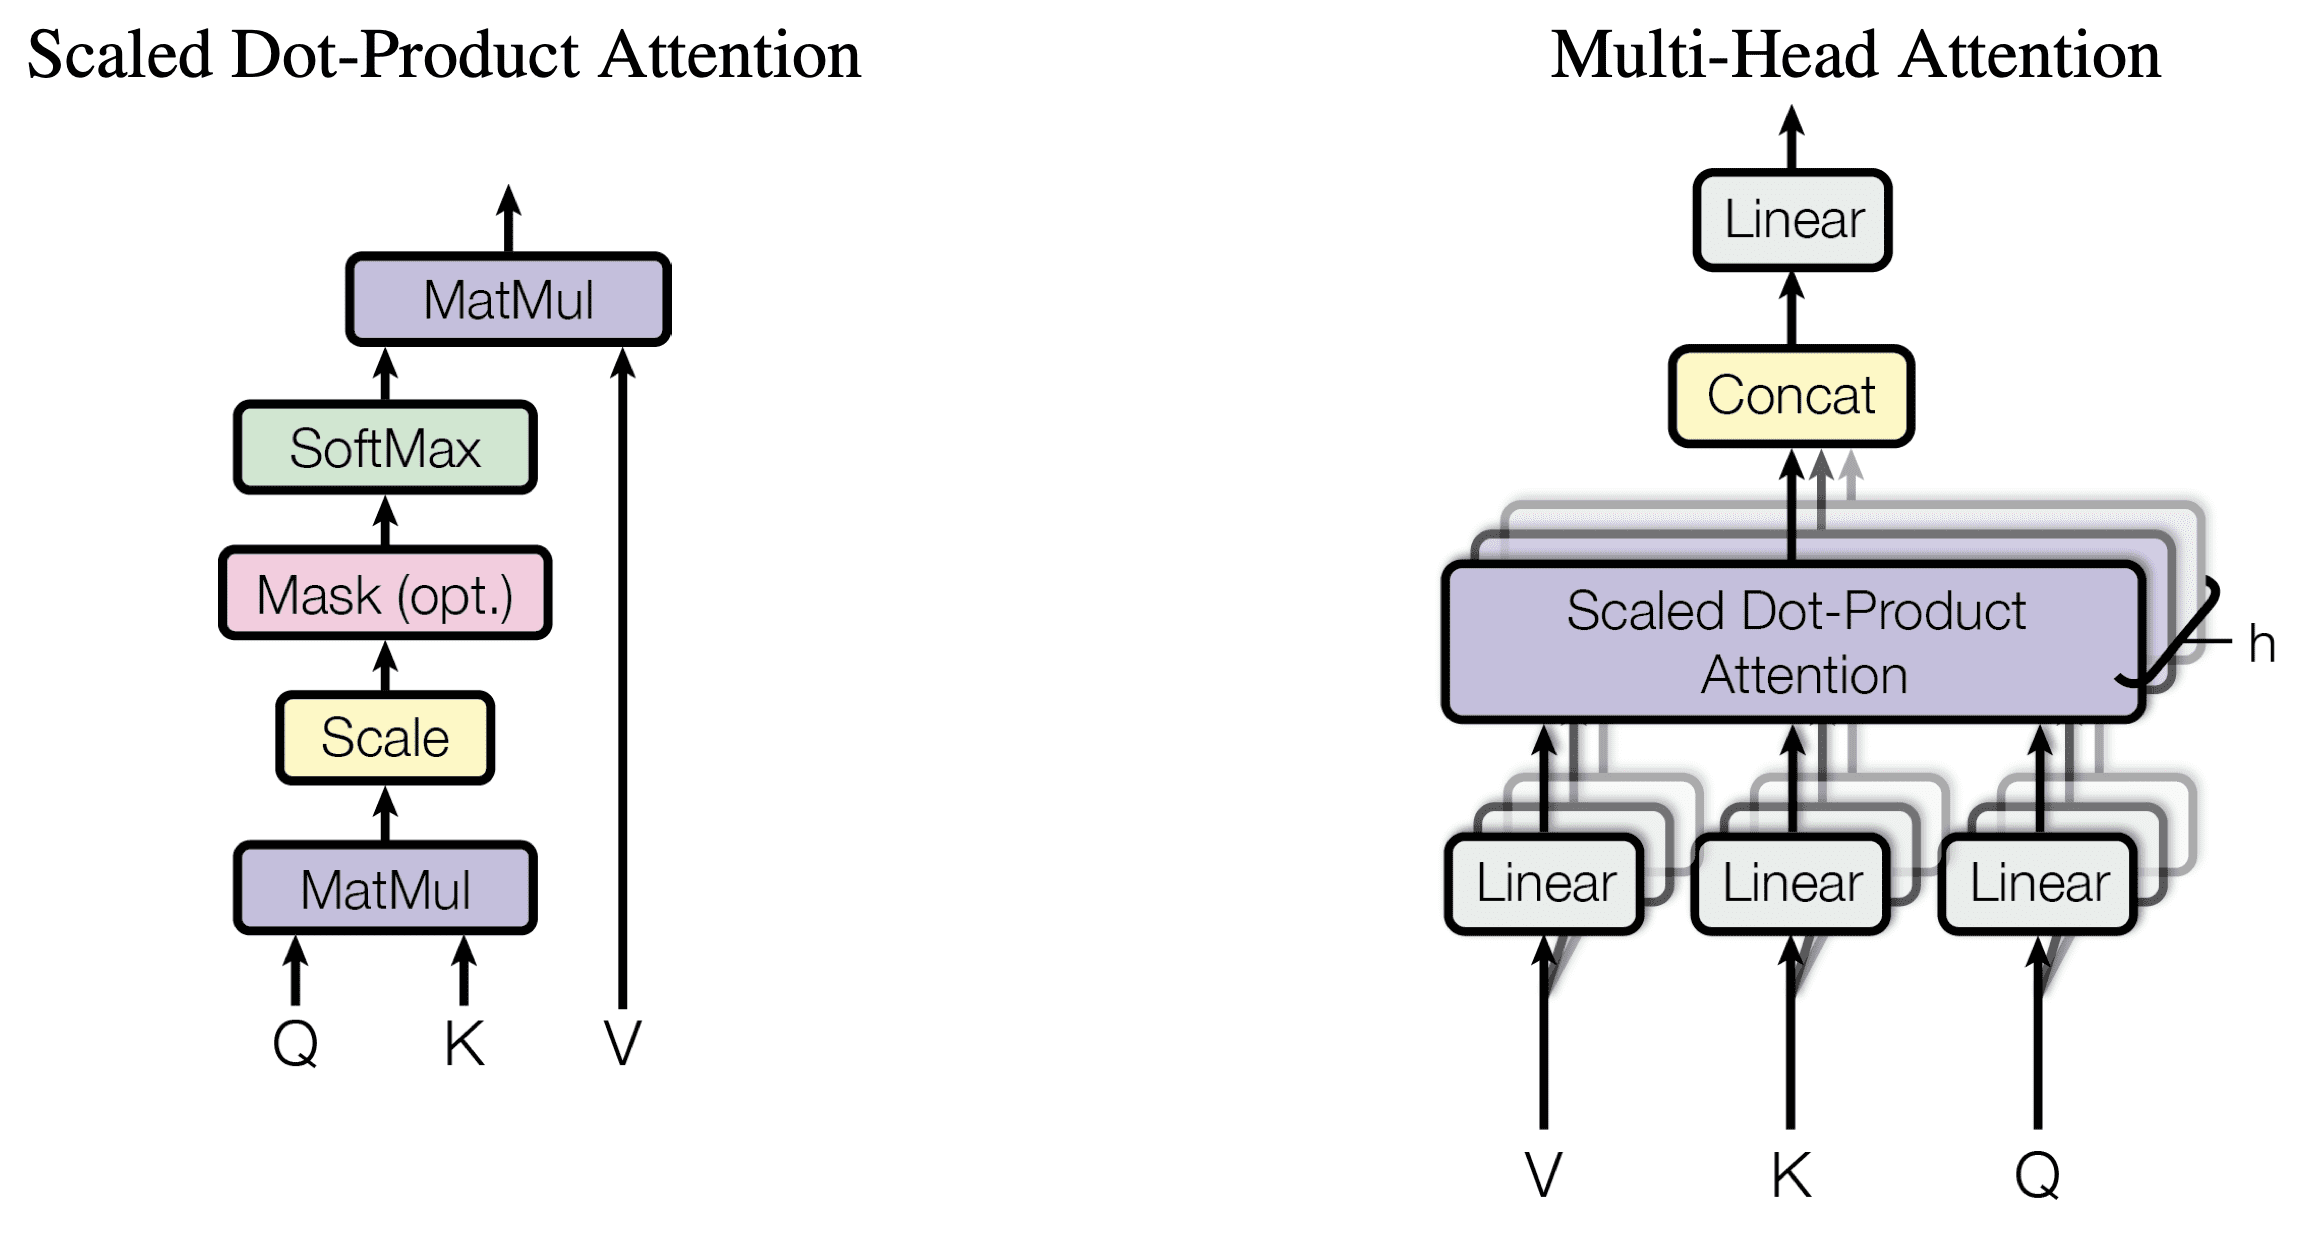
\includegraphics[scale=0.15]{scaled_dot_product_attention.png}
    \caption{Scaled Dot-Product Attention and Multi-Head Attention \cite{1706.03762}}
    \label{fig:scaled_dot_product_attention}
\end{figure}




\subsubsection{Linear attention}

In \cite{2006.16236}, authors propose an extension to the dot-product attention mechanism called \textbf{linear attention}.
This significantly reduces the computational complexity of the attention mechanism by eliminating the need to compute the softmax function.

Notice that in \ref{eq:dot_product_attention_matrix}, the softmax function is applied rowwise to the matrix $Q K^T$.
The softmax function can be substituted with a general similarity function $\text{sim}(\cdot, \cdot)$ between a query $q_i$ and a key $k_j$.
The equation \ref{eq:dot_product_attention_matrix} for output value $v'_i$ can then be rewritten as follows:
\begin{equation}
    v'_i=\text{Attention}(Q, K, V)_i=\frac{\sum_j \text{sim}(q_i, k_j) v_j}{\sum_j \text{sim}(q_i, k_j)}
\end{equation}

% TODO: maybe explain the kernel trick...
% https://en.wikipedia.org/wiki/Kernel_method
The only constrained imposed on the similarity function $\text{sim}(\cdot, \cdot)$ is that it should be non-negative for it to define an attention function.
This conveniently includes all kernels. That is $\text{sim}(q_i, k_j)=\phi(q_i)^T \phi(k_j)$ where $\phi(\cdot)$ is a feature map.

So that given a kernel with a feature map $\phi(\cdot)$, the attention mechanism can be computed as follows:
\begin{equation}
    v'_i=\text{Attention}(Q, K, V)_i=\frac{\sum_j \phi(q_i)^T \phi(k_j) v_j}{\sum_j \phi(q_i)^T \phi(k_j)}
\end{equation}

And we can rewrite the attention mechanism in matrix form as follows:
\begin{equation}
    \text{Attention}(Q, K, V)=\frac{\phi(Q)^T \phi(K) V}{\phi(Q)^T \phi(K)}
\end{equation}

Regrouping the terms, we get the following expression for the attention mechanism:
\begin{equation}
    \text{Attention}(Q, K, V)=\phi(Q)^T \frac{\phi(K) V}{\phi(Q)^T \phi(K)}
\end{equation}

% TODO: maybe rewrite with an example so that it is even more evident for the reader?...
which makes it evident that we can compute $\sum_j \phi(k_j) v_j$ once and reuse them for all the queries $q_i$
which reduces the computational complexity from $O(N^2)$ to $O(N)$ where $N$ is the number of input vectors
in the attention layer.

\begin{remark}
    In \cite{2006.16236}, authors used the $\phi(x)=elu(x)+1$ feature map where
    $elu(x)=\max(0, x)+\min(0, \alpha(\exp(x)-1))$ is the exponential linear unit activation function.
    This feature map is used to ensure that the attention mechanism is non-negative
    and hence defines a valid attention function. Moreover, $elu(\cdot)$ is used instead of $ReLU(\cdot)$
    to ensure the differentiability when x is negative.
\end{remark}


% TODO: compare to other competitors for attention layer
% https://uvadlc-notebooks.readthedocs.io/en/latest/tutorial_notebooks/tutorial6/Transformers_and_MHAttention.html
% convolutional, etc.


% TODO: different architectures from lilian weng blog, retformer, the TF in TS survey.
% describe different attention mechanisms
% https://uvadlc-notebooks.readthedocs.io/en/latest/tutorial_notebooks/tutorial6/Transformers_and_MHAttention.html
% http://nlp.seas.harvard.edu/annotated-transformer/
% https://peterbloem.nl/blog/transformers
% lilian weng


\subsection{Transformers for time series modelling}

TODO: provide the main overview of the papers that use transformers for time series modelling,
the comparison to other methods, the comparison of different transformer architectures specifically
tailored for time-series


%%%%%%%%%%%%%%%%%%%%%%%%%%%%%%%%%%%%%%%%%%%%%%%
\section{FPGA design}

% Main xilinx docs:
% https://docs.xilinx.com/r/en-US/ug1399-vitis-hls/Summary?tocId=xCTL3tR5AjP_FFYmRfl81Q

In this section, the main design principles of programming an FPGA board will be described. Readers will be introduced to the common optimization techniques and how they are achieved. The FPGA programming will be done using C++ HLS which is converted to verilog code.

\subsection{Introduction to FPGA}

% for efficient implementation reference:
% https://pytorch.org/tutorials/intermediate/scaled_dot_product_attention_tutorial.html?utm_source=whats_new_tutorials&utm_medium=scaled_dot_product_attention_tutorial

% TODO: maybe rewrite
The progress of hardware acceleration devices like field-programmable gate arrays (FPGAs) enables the achievement of high component density and low power consumption, all the while minimizing latency \cite{10.1007/978-3-319-56258-2_14}. They are commonly used to accelerate high-performance, computationally intensive systems (for example, data centers) or to minimize the latency of execution (for example, in high-frequency trading).

\subsection{FPGA development} \label{sec:fpga_development}

\subsubsection{Common Terms}

In this section, common terms will be introduced.
The terms will be used throughout Section \ref{sec:fpga_development}.
It is not required to read all of them at once, but it is recommended to refer to this section
when a term is not clear and the reader can refer to this section when necessary.

\begin{definition}
    \textbf{LUT (Look-Up Table)} is a small, fast memory that stores the output of a Boolean function of its inputs.
    The LUT is the basic building block of an FPGA and is capable of implementing any logic function of N Boolean variables.
\end{definition}
\begin{definition}
    \textbf{BRAM (Block RAM)} is a dedicated two-port memory that can be used to store data.
\end{definition}
\begin{definition}
    \textbf{Clock cycle} is the time between two consecutive rising edges of the clock signal.
    It is the amount of time between two pulses of an oscillator, a single increment of the
    central processing unit (CPU) clock during which the smallest unit of processor activity
    is carried out.
\end{definition}
\begin{definition}
    \textbf{Latency} is the time between the start of an operation and the moment its results become available
    or the number of clock cycles required to complete an operation.
    \textbf{Latency of a loop} is the number of clock cycles required to complete one iteration of the loop.
\end{definition}
\begin{definition}
    \textbf{Throughput} is the number of operations that can be completed in a given amount of time.
\end{definition}
\begin{definition}
    \textbf{Initiation Interval (II)} is the number of clock cycles between the start of two consecutive iterations of a loop.
    That is, it is the maximum rate (in clock cycles) at which loop iterations can be initiated.
    In the ideal case, the II is equal to 1 so that we can start a new iteration of the loop every clock cycle.
    Initiation interval is different from latency.
    The reason for this is pipelining which will be described in Section \ref{sec:pipelining}.
    For a visual explanation, see Figure \ref{fig:latency_vs_ii}.
\end{definition}
\begin{definition}
    \textbf{Trip count} is simply the number of iterations of a loop.
\end{definition}

\begin{figure}[h!]
    \centering
    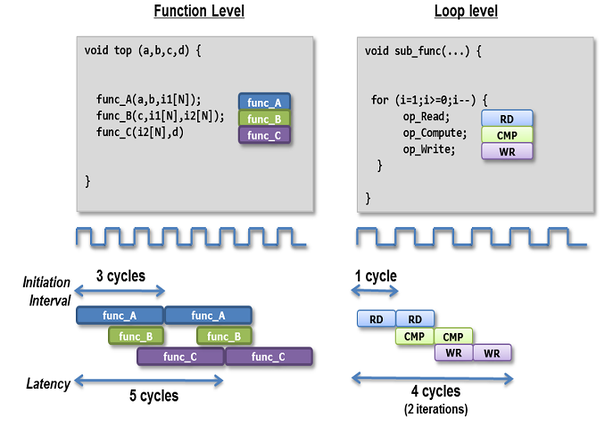
\includegraphics[scale=0.7]{iiandlatency.png}
    \caption{Latency vs Initiation Interval illustration. Source: \cite{VitisYork}}
    \label{fig:latency_vs_ii}
\end{figure}

\subsubsection{HLS synthesis} \label{sec:hls_synthesis}

In this section, HLS synthesis will be described ~\cite{AMD2023VitisHLS}.
It is now the common workflow in the FPGA development because it significantly
improves the productivity when working with design.

HLS synthesis is a methodology that bridges the gap between high-level programming
languages, such as C, C++, or OpenCL, and the low-level hardware description languages
typically used in FPGA design, like Verilog or VHDL. This approach enables developers
to describe their algorithms and functionality at a higher level of abstraction,
allowing them to focus on the problem-solving aspect rather than the intricacies of hardware implementation.

The HLS process starts with a high-level description of the desired functionality.
This description can be written in familiar programming languages (in this case, C++ HLS),
taking advantage of their abstractions and concise syntax.
The HLS tool then performs a series of transformations on this high-level description to generate
an optimized hardware implementation that can be deployed on an FPGA.
The high-level description is transformed by the HLS tool into a RTL (Register Transfer Level) representation,
which is the low-level hardware description that defines the behavior of the FPGA.


\subsubsection{Simulation, Cosimulation}

In this section, the processes of \textbf{simulation} and \textbf{cosimulation} will be described.
In the context of developing for Field-Programmable Gate Arrays (FPGAs),
simulation and cosimulation are two crucial techniques for verifying and testing the
functionality of your design before actually programming it onto the FPGA hardware.

\begin{definition}
    \textbf{Simulation} is the process of running a software-based model of your FPGA design on
    a computer to simulate its behavior.
    The process is very similar to running a software program on a computer for
    the purpose of unit testing certain parts of functionality of your code
    \cite{AMD2023VitisSimCosim}. That is, the simulation does not
    involve any RTL code and is simply a software simulation of the high-level description..
\end{definition}

\begin{remark}
    Simulation might not always capture all aspects of hardware behavior, such as timing delays, which can be critical on FPGAs.
\end{remark}

\begin{definition}
    \textbf{Cosimulation} is a technique that combines simulation of the high-level description with simulation of the generated RTL description.
    This means that the simulations of both the original high-level code and the RTL representation in parallel, comparing their behavior.
    The purpose of cosimulation is to ensure that the high-level synthesis tool accurately transformed the high-level description into the desired RTL behavior.
    \cite{AMD2023VitisSimCosim}.
\end{definition}


\subsection{Common optimizations}

In this section, common optimization techniques and how they are achieved will be introduced.

It is quite common to process data blocks
(for example, a sequence of samples in anomaly detection) using for loops.
For loops are usually the main bottleneck in the performance of the design
and it is the area where most of the optimizations are applied first \cite{AMD2023VitisHLS}.


\subsubsection{Loop Pipelining} \label{sec:loop_pipelining}

% sounds very general to me....
Loop pipelining is a technique used in FPGAs programming to optimize the performance of sequential operations within a loop.
It improves the throughput of loops by breaking them down into multiple stages
that can execute concurrently.
That is, it allows to start the next iteration of a loop before the current
iteration has finished \cite{AMD2023Pipelining}.
Refer to Figure \ref{fig:loop_pipelining} and Figure \ref{fig:latency_vs_ii} for a visual illustration.

% also good examples here
% https://wiki.york.ac.uk/display/RTS/Practical+4+-+Vitis+HLS


\begin{figure}[h!]
    \centering
    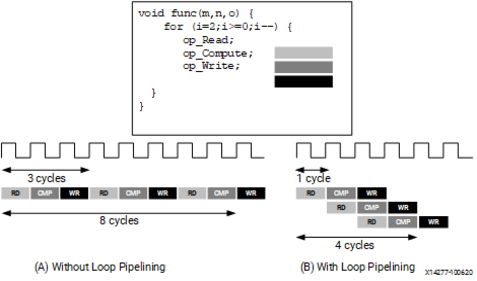
\includegraphics[scale=0.7]{loop_pipelining.png}
    \caption{Loop pipelining illustration. Source: \cite{AMD2023Pipelining}}
    \label{fig:loop_pipelining}
\end{figure}


% TODO: maybe just leave it as normal text without using \begin{exa}
% the style is a bit strange...
\begin{exa}
    Consider example of pipelining a simple for loop which adds 2 vectors (\cite{AMD2023Pipelining}):
    \begin{lstlisting}[language=c++,numbers=none]
void toplevel(int* a, int* b, int* c, int len) {
	vadd: for(int i = 0; i < len; i++) {
#pragma HLS PIPELINE
	   c[i] = a[i] + b[i];
	}
}
\end{lstlisting}

    Taking the reference numbers from \cite{AMD2023Pipelining},
    assume that len is 20 and that one loop iteration takes 3 clock cycles,
    then the total latency of the loop is 60 clock cycles without pipelining.

    The pipelining pragma \texttt{\#pragma HLS PIPELINE} allows to start
    the next iteration of the loop before the current iteration has finished.

    By default, the pipelining pragma will try to achieve an II of 1 but this
    can be specified manually by using the \texttt{II} parameter.

    % a dumb simple example of calculations: https://support.xilinx.com/s/question/0D52E00006hprvzSAA/hls-loop-pipeline-and-iteration-latency?language=en_US
    % and also a dumb example with formula for different II: https://www.intel.com/content/www/us/en/docs/programmable/683152/21-3/pipeline-loops.html
    So, the pipelining pragma reduces the latency of the loop to 22 clock cycles.

    In general, the latency of a loop with pipelining is given by the following formula:
    \begin{equation}
        \text{Latency} = \text{II} \cdot (\text{Trip Count} - 1) + \text{Loop Body Latency}
    \end{equation}
\end{exa}

\begin{remark}
    It is not always possible to achieve an II of 1.
    This is because of the dependencies between the iterations of the loop.
    For example, if the loop body depends on the result of the previous iteration,
    then the II cannot be 1 and we have to wait until the previous iteration has finished
    before starting the next one.
\end{remark}

% good description of 
% https://docs.xilinx.com/r/en-US/ug1399-vitis-hls/Loops-Primer


\subsubsection{Loop Unrolling}

Loop unrolling is an optimization technique that involves expanding or unwinding
loops in code to potentially enable better utilization of hardware resources and/or
to minimize control flow (branching) in loop iterations.
This technique is not limited to FPGA development but can be particularly useful
in optimizing code for FPGA implementations.

Loop unrolling works by duplicating loop iterations (read as \texttt{copy-pasting}).
This allows utilizing more hardware as the loop body is duplicated multiple times
and loop iterations will utilize different hardware resources.
This increase in performance (i.e., throughput) comes at the cost of increased
resource utilization \cite{AMD2023Pipelining}.

\begin{exa}
    Consider a simple example of a function which multiplies the
    input vector of length 4 by a constant, 2:
    \begin{lstlisting}[language=c++,numbers=none]
void toplevel(int* a, int* b) {
	smult: for(int i = 0; i < 4; i++) {
#pragma UNROLL
	   b[i] = 2 * a[i];
	}
}
\end{lstlisting}

    The unroll pragma \texttt{\#pragma UNROLL} allows to unroll the loop and execute
    the loop iterations in parallel.

    The unrolled version of the loop will be equivalent to the following code:

    \begin{lstlisting}[language=c++,numbers=none]
void toplevel(int* a, int* b) {
	b[0] = 2 * a[0];
	b[1] = 2 * a[1];
	b[2] = 2 * a[2];
	b[3] = 2 * a[3];
}
\end{lstlisting}

\end{exa}

\begin{remark}
    It might not be possible to unroll a loop.
    For example, if the trip count is not known at compile time then the loop cannot be unrolled.
    Sometimes it is possible to unroll a loop partially. The unroll pragma allows to specify
    the factor of unrolling, i.e., how many iterations to unroll.
    For example, \texttt{\#pragma UNROLL factor=2} will only duplicate the loop body
    so that there are 2 of them.
\end{remark}

% TODO: Loop Pipelining and unrolling
% TODO: nested loops behaviour (see loop pipelining section)

\subsubsection{Function Inlining}

% not specific to FPGA, but can be useful
% https://wiki.york.ac.uk/display/RTS/Practical+4+-+Vitis+HLS


% good example of array partition:
% https://github.com/twaclaw/matmult/tree/master

% good guide:
% https://wiki.york.ac.uk/display/RTS/Vitis+HLS+Knowledge+Base

\subsubsection{Arrays}
% https://docs.xilinx.com/r/en-US/ug1399-vitis-hls/Arrays-Primer
% https://docs.xilinx.com/r/en-US/ug1399-vitis-hls/Array-Accesses-and-Performance

TODO: Partitioning (block, cyclic, complete)

\subsubsection{Streams}

TODO:

% https://docs.xilinx.com/r/en-US/ug1399-vitis-hls/Arrays-on-the-Interface

% https://docs.xilinx.com/r/en-US/ug1399-vitis-hls/Memory-Mapped-Interface

% https://docs.xilinx.com/r/en-US/ug1399-vitis-hls/Optimizing-AXI-System-Performance


\subsubsection{Example of optimized matrix multiplication}


% this is quite a cool video that goes into the details
% https://www.youtube.com/watch?v=JeERDmY2qkU

% biggest problem: partitioning the B array if pipeline the outer loop
% good choice - j loop because you combine the pipeline + partition
% + loop unrolling (implied)

% then: more efficient partitioning (or reshaping) trick


% TODO: performance metric

% maybe add as further steps blocked matrix mult
% but don't need to do it here because it fits into memory
% anyway
% maybe also add vector types hls::vector<DTYPE, DSIZE>
% TODO: transpose matrix A before for vector types (so that can fetch at consecutive address)


%%%%%%%%%%%%%%%%%%%%%%%%%%%%%%%%%%%%%%%%%%%%%%%
\chapter{Experiments}


\section{Architecture and hyperparameters}

% use simple gridsearch + plot evaluation metrics

Here we will describe the model architecture and the hyperparameters used for the experiments.

In the experiments 3 models were used for comparison:
\begin{itemize}
    \item \textbf{Linear Regression} - a simple linear regression model on handcrafted features
    \item \textbf{Transformer Encoder} - a transformer encoder model on raw time series data
    \item \textbf{Linear Transformer Encoder} - a linear transformer model on raw time series data
\end{itemize}

For both transformer models, we used the encoder architectures as described in Section \ref{sec:attention_mechanism}
with a linear layer on top of the output of the transformer encoder to get the final prediction (i.e., if a sample is an anomaly).
\begin{remark}
    The encoder part has positional encoding and layer normalization disabled.
    We found that the positional encoding does not improve the performance of the model and leads to more
    unstable training (see Section \ref{sec:training}).
\end{remark}

The transformer hyperparameters used for the experiments are presented in Table \ref{tab:hyperparameters}.

% TODO: this might change in the future if I find a better architecture
\begin{table}[h!]
    \centering
    \begin{tabular}{|c|c|c|c|c|}
        \hline
        Parameter, Model            & Transformer Encoder & Linear Transformer Encoder \\
        \hline
        Window Size                 & 8                   & 8                          \\
        Number of heads             & 8                   & -                          \\
        Dim. of FeedForward network & 16                  & 16                         \\
        Number of blocks            & 2                   & 1                          \\
        \hline
    \end{tabular}
    \caption{Hyperparameters}
    \label{tab:hyperparameters}
\end{table}

The learning rate was chosen using the learning rate finder \cite{1506.01186} (see Section \ref{sec:learning_rate_finder})
and the batch size was chosen to be the maximum value that
fitted the dataset in memory ($2^{13}$ samples).


\subsection{Model Fitting} \label{sec:training}

In this section, we will describe the training procedure and the main issues that we encountered and how they were addressed.

\subsubsection{General procedure}

The General process of training a neural network involves iteratively adjusting its
parameters to minimize a specified loss function.
This is typically achieved through an optimization algorithm, such as gradient descent.

That is, at each iteration, the parameters of the model $\theta$ are updated as follows:
\begin{equation} \label{eq:gradient_descent}
    \theta_{t+1}=\theta_t - \alpha \nabla_{\theta} \mathcal{L}(\theta_t)
\end{equation}

where $\alpha$ is the learning rate and $\mathcal{L}(\theta_t)$ is the loss function at the $t$-th iteration.

While the general procedure is simple there are multiple methods to improve the convergence of the optimization algorithm,
which will be described in the following sections.

% TODO: maybe add a section with an optimizer here?

\subsubsection{Learning rate finder} \label{sec:learning_rate_finder}
% describe learning rate finder
The learning rate $\alpha$ is one of the most important hyperparameters that determines the step size in parameter space
during gradient descent optimization. An appropriate learning rate is essential for
model convergence.
The problem of choosing the learning rate is a well-known problem in machine learning
and badly chosen learning rate can lead to either underfitting where the model
learns too slowly or it can lead to divergence where the parameters are updated too abruptly.

In \cite{1506.01186}, authors proposed a simple method to find an appropriate learning rate
automatically by plotting the loss function against the learning rate.

The procedure is performed as follows:
\begin{enumerate}
    \item Start with a very small learning rate $\alpha$ and increase it at each iteration
    \item At each iteration, train the model for a few epochs and compute the loss function
    \item Plot the loss function against the learning rate
          This plot is crucial in identifying the "sweet spot" in the learning rate range
          where the loss is decreasing effectively.
    \item Choose the point on the learning rate vs. loss curve where the
          loss starts to decrease most steeply.  This point indicates that the model
          is making the most significant progress towards convergence.
\end{enumerate}

\begin{remark}
    While there are no guarantees that the learning rate finder will find the optimal learning rate,
    it provides a good empirical estimate of the optimal learning rate.
\end{remark}

Instead of manually plotting the loss function against the learning rate, we used the implementation
provided in Pytorch Lightning \cite{lightning.ai_2023_lr_finder}.


\subsubsection{Gradient explosion and Gradient clipping} \label{sec:gradient_clipping}
A different challenge of training neural networks is the phenomenon known as the "gradient explosion problem."
We have found that the gradient explosion problem is especially prevalent in the proposed architectures.

The gradient explosion problem occurs when the gradient of the loss function with respect to the parameters
becomes too large and the parameters are updated too abruptly (e.g., as in Equation \ref{eq:gradient_descent}).
This can lead to the model diverging and the loss function increasing instead of decreasing.
An example of the loss function diverging is presented in Figure \ref{fig:gradient_explosion}.

\begin{figure}[h!]
    \centering
    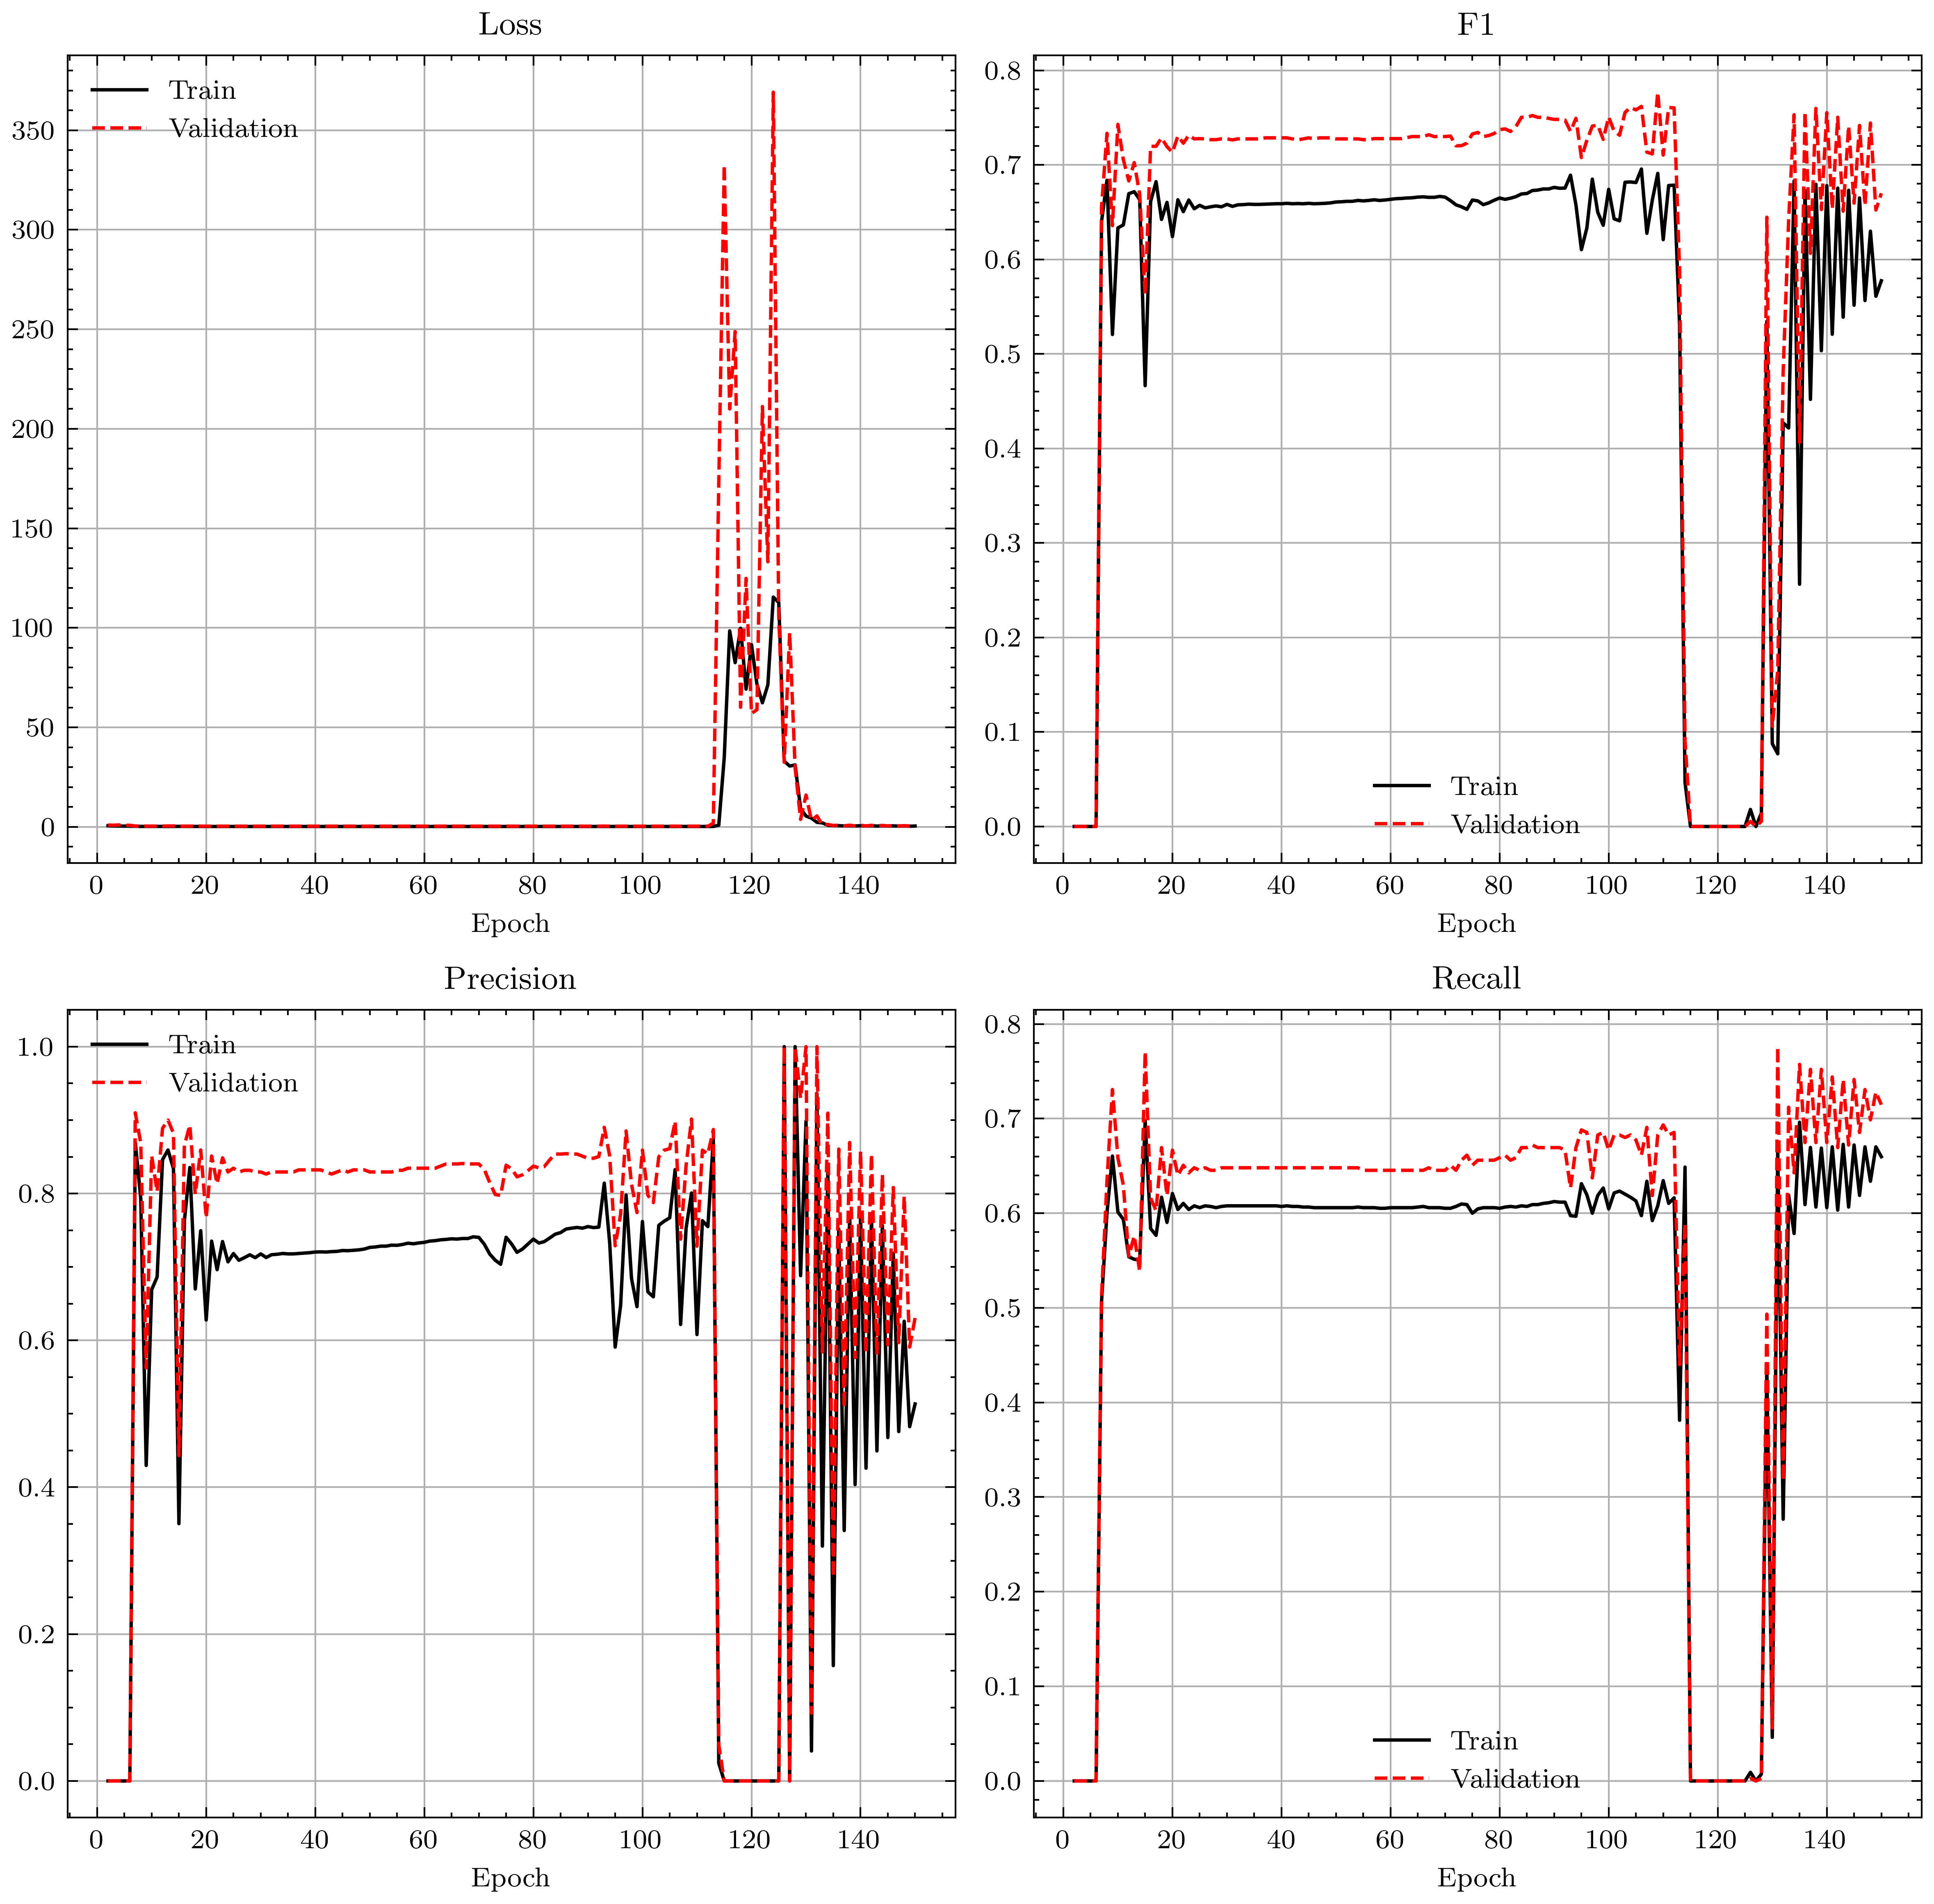
\includegraphics[scale=0.6]{gradient_explosion.png}
    \caption{Example of gradient explosion at around epoch 115 which leads to the loss function diverging for a few following epochs.}
    \label{fig:gradient_explosion}
\end{figure}

To solve the problem of gradient explosion, we used the gradient clipping technique introduced
in \cite{1211.5063}.
The idea behind gradient clipping is to clip the gradient to a maximum value $g_{max}$.
This remediates the problem of gradient explosion because the gradient is bounded and the parameters
are updated more smoothly.

\subsubsection{Class imbalance and loss functions} \label{sec:class_imbalance}

In anomaly detection task the dataset is often imbalanced, i.e., the number of normal samples
is much larger than the number of anomalous samples.

This poses a problem for the training of the model because the model can simply learn to predict
the majority class (i.e., normal samples) and achieve a high accuracy without having
good recall (refer to Section \ref{sec:metrics} for the description to the metrics).

The loss functions that we use for training is the binary cross-entropy loss function
\cite{Good_1952}
which is computed as follows:
\begin{equation} \label{eq:binary_cross_entropy}
    \mathcal{L}(\theta)=-\frac{1}{N} \sum_{i=1}^N y_i \log(\hat{y}_i) + (1-y_i) \log(1-\hat{y}_i)
\end{equation}
where $y_i$ is the true label and $\hat{y}_i$ is the predicted label.

While the binary cross-entropy loss function is a good choice for the anomaly detection task,
it does not take into account the class imbalance problem.

A way to solve the class imbalance problem is to use a weigh positive
samples (i.e., anomalous samples) more than negative samples in the loss function.

So we can modify the loss function as follows:
\begin{equation} \label{eq:weighted_binary_cross_entropy}
    \mathcal{L}(\theta)=-\frac{1}{N} \sum_{i=1}^N w_i (y_i \log(\hat{y}_i) + (1-y_i) \log(1-\hat{y}_i))
\end{equation}
where $w_i$ is the weight of the $i$-th sample.
In the experiments, we found that weighting the positive samples 5 times more than the negative samples
yielded good results for most of the datasets which we used throughout the experiments.

\subsubsection{Training stability: Layer normalization and positional encoding}

While the base transformer encoder architecture uses layer normalization and positional encoding layers,
we found that they lead to unstable training and worse performance of the model on most
of the datasets. Hence, we disabled them for the experiments and replaced them with
identity layers.
% TODO: maybe just add plots with the loss here?

\section{Datasets}

In this section, the datasets used for model training and performance evaluation will be described.

\subsection{Numenta Anomaly Benchmark (NAB)}
To assess the accuracy of predictions, we use the Numenta Anomaly Benchmark ~\cite{Ahmad2017Unsupervised} dataset,
which contains various real-world labeled time series of temperature sensor readings, CPU utilization of cloud machines, service
request latencies, and taxi demands in New York City. It is commonly used to assess the performance of anomaly detection
models on time-series data.

The reason why we use this dataset is that it is a standard benchmark dataset
for anomaly detection in time series and because it has a large number of labeled time series.

A sample time series of NYC taxi demand is presented in Figure \ref{fig:NAB_example_nyc_taxi}.
\begin{figure}[h!]
    \centering
    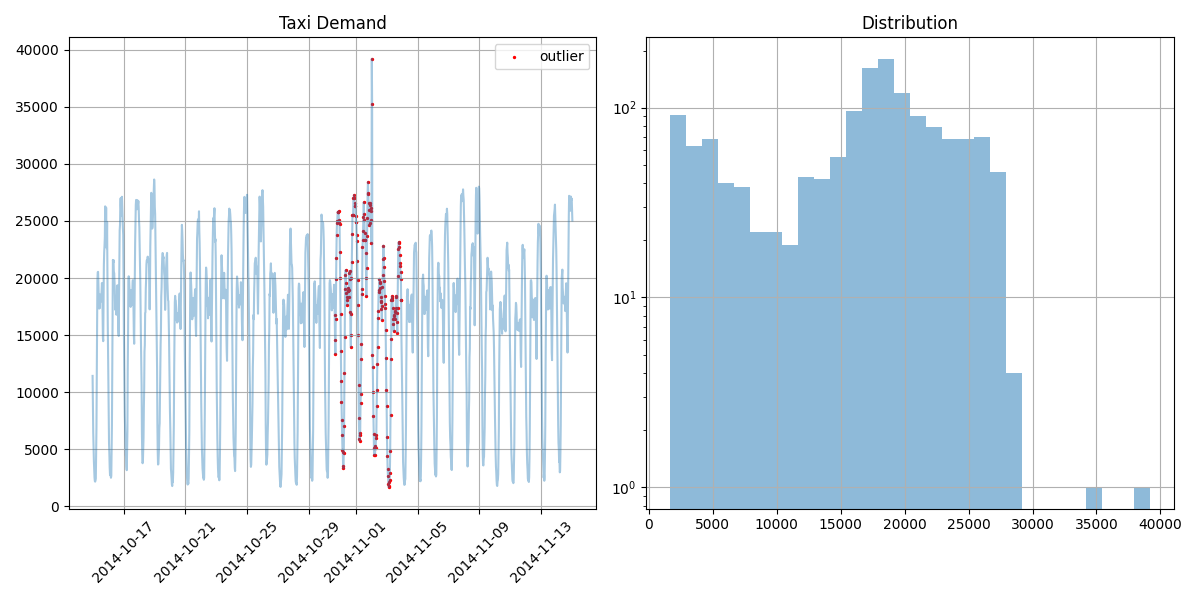
\includegraphics[scale=0.48]{NAB_example_nyc_taxi.png}
    \caption{NYC Taxi demand - anomalies highlighted in red}
    \label{fig:NAB_example_nyc_taxi}
\end{figure}

\subsection{KPI Anomaly Detection Dataset}

The other labeled dataset that we use is the KPI Anomaly Detection Dataset (KPI AIOps) \cite{2208.03938}.
This dataset alongside the NAB dataset will be used to evaluate the predictive performance of the anomaly detection models.

The dataset consists of KPI (key performace index) time series data from many
real scenarios of Internet companies with ground truth label. KPIs fall into two
broad categories: service KPIs and machine KPIs. Service KPIs are performance metrics
that reflect the size and quality of a Web service, such as page response time, page views,
and number of connection errors. Machine KPIs are performance indicators that reflect
the health of the machine (server, router, switch), such as CPU utilization, memory utilization,
disk IO and network card throughput.

A sample time series of a sensor readings is presented in Figure \ref{fig:NAB_example_nyc_taxi}.
We can clearly see the outliers for some of the observations (colored in red).
\begin{figure}[h!]
    \centering
    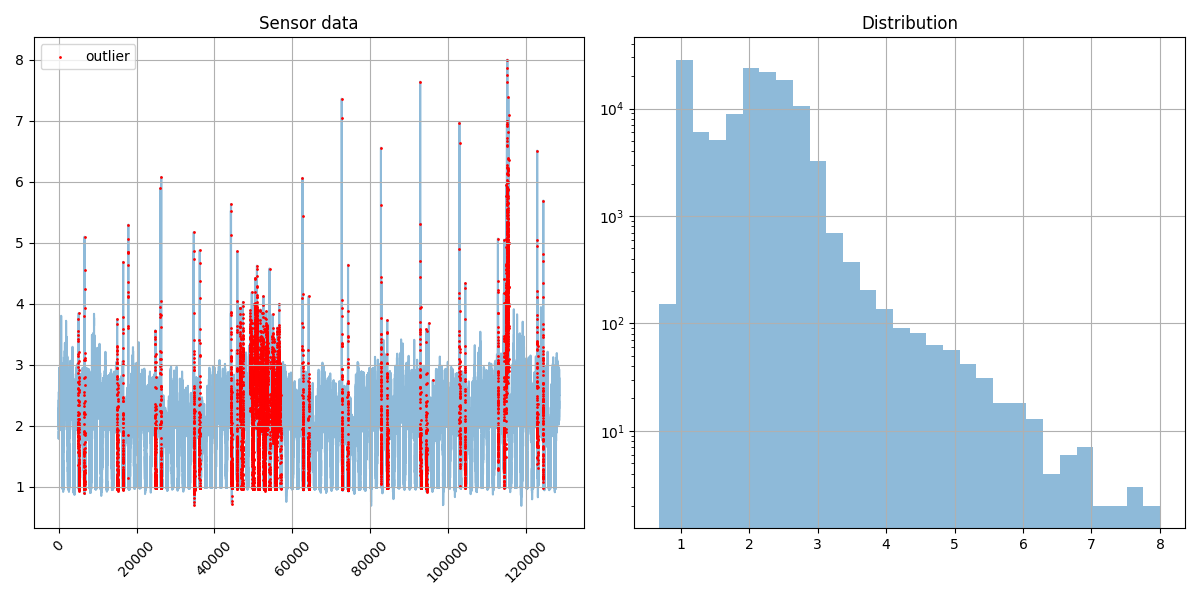
\includegraphics[scale=0.48]{KPIAIOps_example.png}
    \caption{Sensor data from a machine in a data center. The red dots indicate the anomalies.}
    \label{fig:KPIAIOps_example}
\end{figure}

\subsection{FI2010}

In \cite{1705.03233}, authors described the first publicly available benchmark dataset of high-frequency limit order markets for mid-price prediction.
The dataset contains 10-day limit order book data from June 2010 for five stocks that are listed on the Helsinki exchange.
Each entry in the time series provides price details and aggregate order sizes for the top ten levels on both the bid and offer sides of the market,
totaling forty data points. The time series consists of approximately four million messages, representing incoming buy/sell orders or cancellations.
The dataset features order book snapshots taken after every 10 messages, resulting in approximately 400,000 records for the five stocks.

A number of versions of the dataset are available using different normalization schemes. We used the not normalized version of the dataset.

For the purpose of this work, we only extract only the mid price from the dataset which will be used for anomaly detection task.


\subsubsection{Synthetic outliers}

Since the dataset is not labeled, we have to inject synthetic anomalies into the dataset.
We employ the approach similar to \cite{Crepey2022Anomaly} with a slight modification.
The algorithm can be summarized as follows:
\begin{enumerate}
    \item Select $n$ samples from the time series which will be contaminated (i.e., anomalous)
    \item Replace the sample $S_i$ with $\hat{S}_i=S_i(1+\delta)$ where $\delta$ is the injected outlier in the return space.
\end{enumerate}

Authors model $\delta$ as a uniformly distributed random variable $\mathcal{U}[0, \rho]$.
We instead use the normal distribution with matching mean and standard deviation of the returns time series.

An example of the injected outliers is presented in Figure \ref{fig:FI2010_example_outliers_injected}
\begin{figure}[h!]
    \centering
    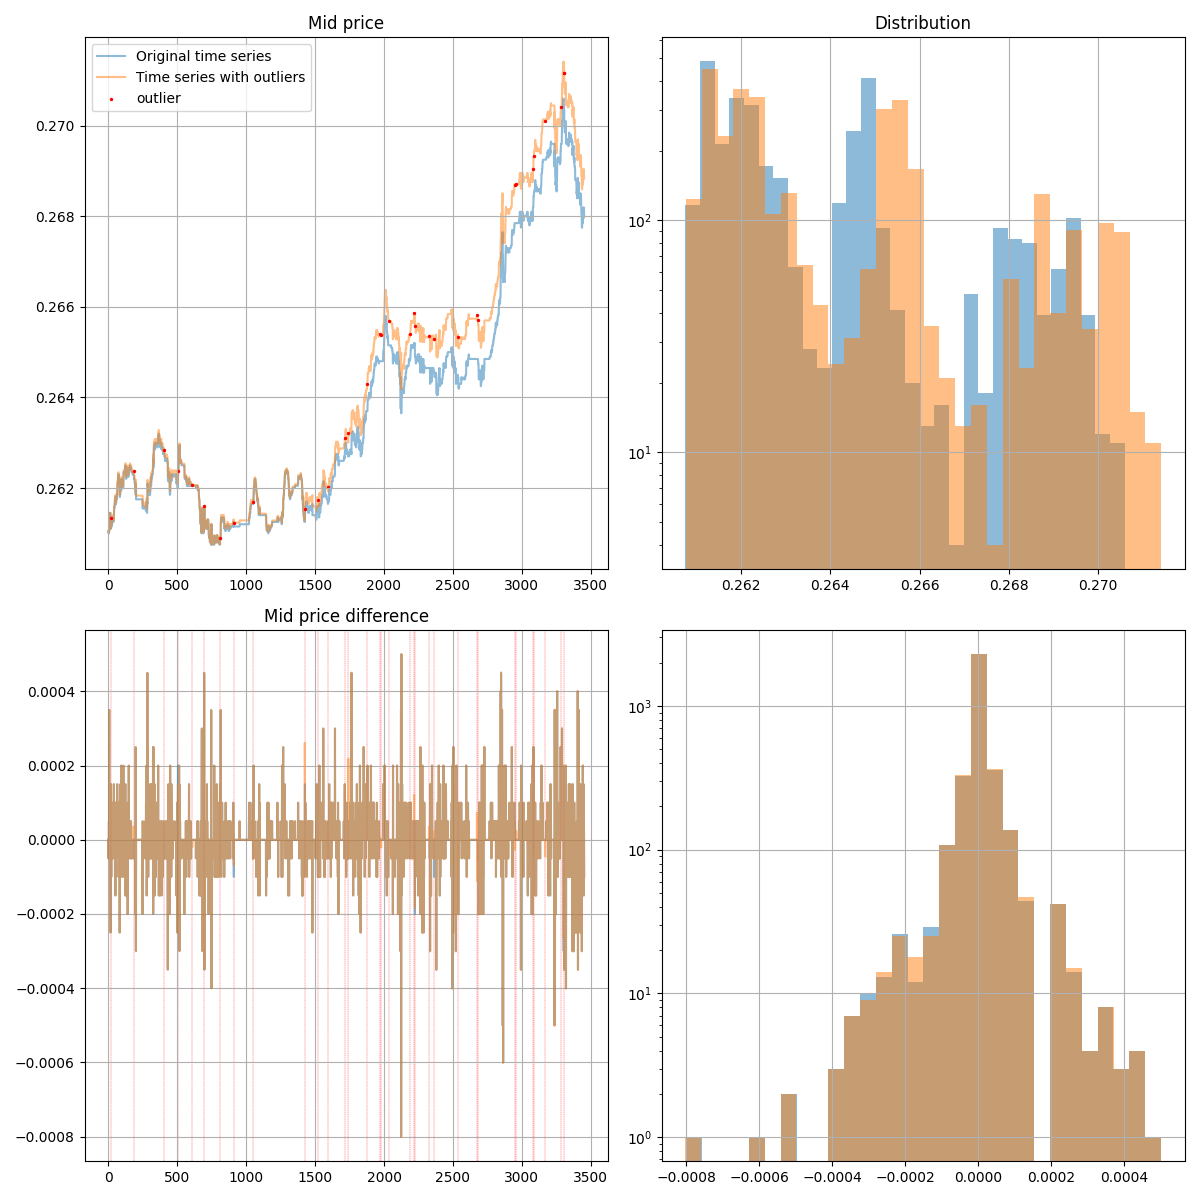
\includegraphics[scale=0.48]{FI2010_example_outliers_injected.png}
    \caption{Example of the injected outliers in the FI2010 dataset.}
    \label{fig:FI2010_example_outliers_injected}
\end{figure}

\section{Accuracy}

% TODO: maybe add citations? or is it a common knowledge

In this section, we will describe the main metrics used to evaluate the performance of the anomaly detection models.
The Transformer encoder model will be compared with the simple linear regression model on handcrafted features
and with the Linear Transformer model \cite{2006.16236}.
The inference procedure will be described and the results will be presented.

\subsection{Inference}
After training the model on the training set as described in Section \ref{sec:training}, we can use the model to make predictions on the test set.

\subsection{Metrics} \label{sec:metrics}

In this section the metrics used to evaluate the performance of the anomaly detection models will be described.

Before we describe the metrics, we need to introduce the confusion matrix and
the following notation:
\begin{itemize}
    \item \textbf{TP} - True Positive calculated as the number of correctly predicted anomalies
    \item \textbf{TN} - True Negative calculated as the number of correctly predicted non-anomalies
    \item \textbf{FP} - False Positive which is the number of incorrectly predicted anomalies
    \item \textbf{FN} - False Negative which is the number of incorrectly predicted non-anomalies
    \item \textbf{P} - Number of positive samples, i.e., $\textbf{P}=\textbf{TP}+\textbf{FN}$
    \item \textbf{N} - Number of negative samples, i.e., $\textbf{N}=\textbf{TN}+\textbf{FP}$
\end{itemize}

The confusion matrix is a table with two rows and two columns that reports the number of false positives, false negatives, true positives, and true negatives.

% https://tex.stackexchange.com/a/20274
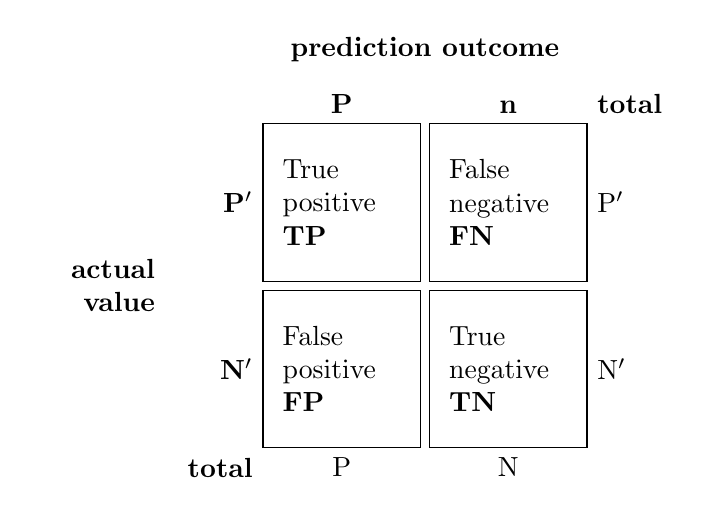
\begin{tikzpicture}[
        box/.style={draw,rectangle,minimum size=2cm,text width=1.5cm,align=left}]
    \matrix (conmat) [row sep=.1cm,column sep=.1cm] {
        \node (tpos) [box,
            label=left:\( \mathbf{P'} \),
            label=above:\( \mathbf{P} \),
        ] {True \\ positive \textbf{TP}};
         &
        \node (fneg) [box,
            label=above:\textbf{n},
            label=above right:\textbf{total},
            label=right:\( \mathrm{P}' \)
        ]{False \\ negative \textbf{FN}};
        \\
        \node (fpos) [box,
            label=left:\( \mathbf{N'} \),
            label=below left:\textbf{total},
            label=below:P
        ] {False \\ positive \textbf{FP}};
         &
        \node (tneg) [box,
            label=right:\( \mathrm{N}' \),
            label=below:N
        ] {True \\ negative \textbf{TN}};
        \\
    };
    \node [left=.05cm of conmat,text width=1.5cm,align=right] {\textbf{actual \\ value}};
    \node [above=.05cm of conmat] {\textbf{prediction outcome}};
\end{tikzpicture}

The matrix summarizes the predictions from a classification model, i.e.,
how well the model performed when predicting the class labels for positive
and negative samples.
While the matrix presents the most informative view of the performance of the model,
we still need to summarize the information in the matrix into a single number(s)
that can be used to compare different models.

In this paper, we will use the following metrics to compare the performance of the anomaly detection models:

\begin{itemize}
    \item \textbf{Accuracy} is the fraction of predictions that the model got right.
          It is defined as follows:
          $$\text{Accuracy}=\frac{\textbf{TP}+\textbf{TN}}{\textbf{TP}+\textbf{TN}+\textbf{FP}+\textbf{FN}}$$
          While this metric is easy to understand, it is not very informative when the dataset is imbalanced
          which is the case for the anomaly detection task where the proportion
          of positive samples is low.

    \item \textbf{Precision} is the fraction of positive predictions that were correct.
          $$\text{Precision}=\frac{\textbf{TP}}{\textbf{TP}+\textbf{FP}}$$
          This metric is useful when the cost of false positives is high.
          For example, in the case of anomaly detection, we want to have
          a high precision so that we do not have to manually check many false positives
          or trigger any downstream filtering task too often.

    \item \textbf{Recall} is the fraction of positive samples that were correctly predicted.
          $$\text{Recall}=\frac{\textbf{TP}}{\textbf{TP}+\textbf{FN}}$$
          This metric is useful when the cost of false negatives is high.
          For example, in the case of anomaly detection, we want to minimize the number of false negatives
          because we do not want to miss any anomalies.

    \item \textbf{F1} is the harmonic mean of precision and recall which ranges from 0 to 1.
          $$\text{F1}=2\cdot\frac{\text{Precision}\cdot\text{Recall}}{\text{Precision}+\text{Recall}}$$
          This metric is useful when we want to balance the precision and recall.
          For example, in the case of anomaly detection, we want to have a high precision
          so that we do not have to manually check many false positives
          or trigger any downstream filtering task too often.
          At the same time, we want to minimize the number of false negatives
          because we do not want to miss any anomalies.

          The advantage of using this metric instead of the accuracy is that it
          can be used even when the dataset is highly imbalanced and it would
          detect if the model performs poorly in terms of precision and/or recall.
\end{itemize}


\subsection{Comparison}

% for metrics example: https://www.mdpi.com/1999-4893/15/10/385`'
% or this: https://thesis.unipd.it/retrieve/840738c1-c175-4529-b5e5-795b393a36a2/Baron_Alex.pdf

\section{Performance/Speed}

% https://xilinx.github.io/Vitis-Tutorials/2021-2/build/html/docs/Getting_Started/Vitis_HLS/dataflow_design.html

% why pynq has additional latency
% https://discuss.pynq.io/t/execution-time-in-pynq-z2/2833
% https://discuss.pynq.io/t/execution-time-calculation/1959
% In pipeline designs there are two key concepts
% Initiation Interval (II), the number of clock cycles between the start times of consecutive loop iterations, ideally this should be 1
% Latency, the time it takes to get an output since the input was fed



\section{Resource utilization on FPGA}



%%%%%%%%%%%%%%%%%%%%%%%%%%%%%%%%%%%%%%%%%%
\newpage
\chapter*{Conclusion}

\section{Future work}
Bigger FPGA boards.

Evaluation of performance on more recent financial market data.


%%%%%%%%%%%%%%%%%%%%%%%%%%%%%%%%%%%%%%%%%%%%%%%
%%%%%%%%%%%%%%%%%%%%%%%%%%%%%%%%%%%%%%%%%%%%%%%
\newpage
\appendix
\chapter{Code}
\section{Efficient matrix multiplication}\label{app:Appendix}
This is Appendix~\ref{app:Appendix}, which usually contained supporting material,
or complicated proofs that might make the main text above less readable / fluid.

%%%%%%%%%%%%%%%%%%%%%%%%%%%%%%%%%%%%%%%%%%%%%%%
%%%%%%%%%%%%%%%%%%%%%%%%%%%%%%%%%%%%%%%%%%%%%%%
\bibliographystyle{unsrt}
\bibliography{biblio}
\addcontentsline{toc}{chapter}{Bibliography}

\end{document}